\documentclass[twoside]{article}

% We add packages, macros here:
%!TEX root =  lec-template.tex
\usepackage{lmodern}
\usepackage[english]{babel}
\usepackage{latexsym}
\usepackage{amsmath}
\usepackage{mathrsfs}
\usepackage{amssymb}
\usepackage{mathtools}
\usepackage[inline,shortlabels]{enumitem} % we prefer enumitem because of its margin adjustment caps
\usepackage{bm}
\usepackage{datetime}
\usepackage[table,xcdraw]{xcolor}
\usepackage{accents}
\usepackage{tikz}
\usepackage{listings}
\usepackage{mdframed}
\usepackage{pgfplots}
\usepackage{pgfplotstable}
\usepackage[boxed]{algorithm}
\usepackage{algpseudocode}
\usepackage{dsfont}
\usepackage{color}
\usepackage{colortbl}
\usepackage{pifont}
\usepackage[bf,font=small,singlelinecheck=off]{caption}
\usepackage{microtype} % improved spacing between words for easier reading
\usepackage{float}
\usepackage{xfrac} % sfrac
\usepackage{xspace}

\linespread{1.1}


\usepackage[textsize=tiny]{todonotes}
\makeatletter
\renewcommand{\todo}[2][]{\@todo[#1]{#2}}
\makeatother

\setlength{\marginparwidth}{10ex}
\newcommand{\todoc}[2][]{\todo[size=\scriptsize,color=blue!20!white,#1]{Csaba: #2}}
\newcommand{\todoj}[2][]{\todo[size=\scriptsize,color=red!20!white,#1]{Jincheng: #2}}

\usepackage{hyperref}
\hypersetup{
    unicode=false,          % non-Latin characters in Acrobat�s bookmarks
    pdftoolbar=true,        % show Acrobat�s toolbar?
    pdfmenubar=true,        % show Acrobat�s menu?
    pdffitwindow=false,     % window fit to page when opened
    pdfstartview={FitH},    % fits the width of the page to the window
    pdftitle={},    % title
    pdfauthor={},     % author
    pdfsubject={Theory, Machine Learning, Lectures},   % subject of the document
    pdfcreator={},   % creator of the document
    pdfproducer={}, % producer of the document
    pdfkeywords={theory} {machine learning} {lecture notes} {CMPUT 654} {Fall 2023}, % list of keywords
    pdfnewwindow=true,      % links in new window
    colorlinks=true,       % false: boxed links; true: colored links
    linkcolor=blue,          % color of internal links (change box color with linkbordercolor)
    citecolor=blue,        % color of links to bibliography
    filecolor=magenta,      % color of file links
    urlcolor=cyan           % color of external links
}
\usepackage{amsthm}
\usepackage{times}
\usepackage{natbib}
\usepackage{nicefrac}
\usepackage{wrapfig}
\usepackage[capitalize]{cleveref}
\usepackage[nottoc,numbib]{tocbibind}

%\usepackage[bmargin=0.75in]{geometry}
\usepackage[margin=1.1in]{geometry}
\usepackage[normalem]{ulem}


%%%%%%%%%%%%%%%%%%%%%%%%%%%%%%%%
% HYPHENATION
%%%%%%%%%%%%%%%%%%%%%%%%%%%%%%%%

\pretolerance=5000
\tolerance=9000
\emergencystretch=0pt
\righthyphenmin=4
\lefthyphenmin=4


\bibliographystyle{plainnat}

\newcommand{\E}{\mathbb{E}}
\newcommand{\EE}[1]{\E[#1]}
\newcommand{\PP}{\mathbb{P}}
\newcommand{\Prob}[1]{\mathbb{P}(#1)}
\newcommand{\one}[1]{\mathbb{I}\{#1\}}
\newcommand{\Supp}{\operatorname{supp}}
\newcommand{\ip}[1]{\langle #1 \rangle}
\newcommand{\bip}[1]{\left\langle #1 \right\rangle}
\newcommand{\norm}[1]{\|#1\|}
\newcommand{\R}{\mathbb{R}}
\newcommand{\N}{\mathbb{N}}
\newcommand{\cA}{\mathcal{A}}
\newcommand{\cB}{\mathcal{B}}
\newcommand{\cC}{\mathcal{C}}
\newcommand{\cD}{\mathcal{D}}
\newcommand{\cE}{\mathcal{E}}
\newcommand{\cF}{\mathcal{F}}
\newcommand{\cG}{\mathcal{G}}
\newcommand{\cH}{\mathcal{H}}
\newcommand{\cK}{\mathcal{K}}
\newcommand{\cL}{\mathcal{L}}
\newcommand{\cN}{\mathcal{N}}
\newcommand{\cP}{\mathcal{P}}
\newcommand{\cQ}{\mathcal{Q}}
\newcommand{\cR}{\mathcal{R}}
\newcommand{\cS}{\mathcal{S}}
\newcommand{\sA}{\mathscr A}

\newcommand{\cM}{\mathcal{M}}
\newcommand{\cX}{\mathcal{X}}
\newcommand{\cY}{\mathcal{Y}}
\newcommand{\NN}{\mathbb{N}}
\newcommand{\RR}{\mathbb{R}}
\newcommand{\VV}[1]{\mathbb{V}[#1]}

\newcommand{\epsapp}{\epsilon}
\newcommand{\epssub}{\delta}

\DeclareMathOperator{\Range}{range}
\newcommand{\rows}{\operatorname{rows}}

\renewcommand{\epsilon}{\varepsilon}
\newcommand{\ceil}[1]{\left\lceil {#1} \right\rceil}
\newcommand{\floor}[1]{\left\lfloor {#1} \right\rfloor}
\newcommand{\ones}{\mathbf{1}}
\newcommand{\zeros}{\mathbf{0}}
\DeclareMathOperator*{\argmin}{arg\ min}
\DeclareMathOperator*{\argmax}{arg\ max}


\def\rvzero{{\mathbf{0}}}
\def\rvone{{\mathbf{1}}}

\def\identiymatrix{\mathbf{Id}}

\newcommand{\softmax}{\mathrm{softmax}}
\newcommand{\KL}{D_{\mathrm{KL}}}

% Graph
\def\gA{{\mathcal{A}}}
\def\gB{{\mathcal{B}}}
\def\gC{{\mathcal{C}}}
\def\gD{{\mathcal{D}}}
\def\gE{{\mathcal{E}}}
\def\gF{{\mathcal{F}}}
\def\gG{{\mathcal{G}}}
\def\gH{{\mathcal{H}}}
\def\gI{{\mathcal{I}}}
\def\gJ{{\mathcal{J}}}
\def\gK{{\mathcal{K}}}
\def\gL{{\mathcal{L}}}
\def\gM{{\mathcal{M}}}
\def\gN{{\mathcal{N}}}
\def\gO{{\mathcal{O}}}
\def\gP{{\mathcal{P}}}
\def\gQ{{\mathcal{Q}}}
\def\gR{{\mathcal{R}}}
\def\gS{{\mathcal{S}}}
\def\gT{{\mathcal{T}}}
\def\gU{{\mathcal{U}}}
\def\gV{{\mathcal{V}}}
\def\gW{{\mathcal{W}}}
\def\gX{{\mathcal{X}}}
\def\gY{{\mathcal{Y}}}
\def\gZ{{\mathcal{Z}}}

% Sets
\def\sA{{\mathbb{A}}}
\def\sB{{\mathbb{B}}}
\def\sC{{\mathbb{C}}}
\def\sD{{\mathbb{D}}}
% Don't use a set called E, because this would be the same as our symbol
% for expectation.
\def\sE{{\mathbb{E}}}
\def\sF{{\mathbb{F}}}
\def\sG{{\mathbb{G}}}
\def\sH{{\mathbb{H}}}
\def\sI{{\mathbb{I}}}
\def\sJ{{\mathbb{J}}}
\def\sK{{\mathbb{K}}}
\def\sL{{\mathbb{L}}}
\def\sM{{\mathbb{M}}}
\def\sN{{\mathbb{N}}}
\def\sO{{\mathbb{O}}}
\def\sP{{\mathbb{P}}}
\def\sQ{{\mathbb{Q}}}
\def\sR{{\mathbb{R}}}
\def\sS{{\mathbb{S}}}
\def\sT{{\mathbb{T}}}
\def\sU{{\mathbb{U}}}
\def\sV{{\mathbb{V}}}
\def\sW{{\mathbb{W}}}
\def\sX{{\mathbb{X}}}
\def\sY{{\mathbb{Y}}}
\def\sZ{{\mathbb{Z}}}

\newcommand{\dimE}{\mathrm{dim}_{\mathcal{E}}}
\DeclareMathOperator{\diam}{diam}


%%
%% ADD PACKAGES here:
%%
%
%\usepackage{amsmath,amsfonts,graphicx}
%
%
% The following commands set up the lecnum (lecture number)
% counter and make various numbering schemes work relative
% to the lecture number.
%

\newcounter{lecnum}
\renewcommand{\thepage}{\thelecnum-\arabic{page}}
\renewcommand{\thesection}{\thelecnum.\arabic{section}}
\renewcommand{\theequation}{\thelecnum.\arabic{equation}}
\renewcommand{\thefigure}{\thelecnum.\arabic{figure}}
\renewcommand{\thetable}{\thelecnum.\arabic{table}}

%
% The following macro is used to generate the header.
%
\newcommand{\lecture}[4]{
   \pagestyle{myheadings}
   \thispagestyle{plain}
   \newpage
   \setcounter{lecnum}{#1}
   \setcounter{page}{1}
   \noindent
   \begin{center}
   \framebox{
      \vbox{\vspace{2mm}
    \hbox to 6.28in { {\bf CMPUT 654 Fa 23: Theoretical Foundations of Machine Learning \hfill Fall 2023} }
       \vspace{4mm}
       \hbox to 6.28in { {\Large \hfill Lecture #1: #2  \hfill} }
       \vspace{2mm}
       \hbox to 6.28in { {\it Lecturer: #3 \hfill Scribes: #4} }
      \vspace{2mm}}
   }
   \end{center}
   \markboth{Lecture #1: #2}{Lecture #1: #2}

   \noindent {\bf Note}: {\it 
   \LaTeX\  template courtesy of UC Berkeley EECS dept. (\href{https://inst.eecs.berkeley.edu/~cs294-8/sp03/Materials/}{link} to directory)
   }

   \noindent {\bf Disclaimer}: {\it These notes have \underline{\textbf{not}} been subjected to the
   usual scrutiny reserved for formal publications. They may be
   distributed outside this class only with the permission of the
   Instructor.} \vspace*{4mm}
}
%
% Convention for citations is authors' initials followed by the year.
% For example, to cite a paper by Leighton and Maggs you would type
% \cite{LM89}, and to cite a paper by Strassen you would type \cite{S69}.
%%%%%%%%% (To avoid bibliography problems, for now we redefine the \cite command.)
%%%%%%%%% Also commands that create a suitable format for the reference list.
%%%%%%%%\renewcommand{\cite}[1]{[#1]}
%%%%%%%%\def\beginrefs{\begin{list}%
%%%%%%%%        {[\arabic{equation}]}{\usecounter{equation}
%%%%%%%%         \setlength{\leftmargin}{2.0truecm}\setlength{\labelsep}{0.4truecm}%
%%%%%%%%         \setlength{\labelwidth}{1.6truecm}}}
%%%%%%%%\def\endrefs{\end{list}}
%%%%%%%%\def\bibentry#1{\item[\hbox{[#1]}]}

%Use this command for a figure; it puts a figure in wherever you want it.
%usage: \fig{NUMBER}{SPACE-IN-INCHES}{CAPTION}
\newcommand{\fig}[3]{
			\vspace{#2}
			\begin{center}
			Figure \thelecnum.#1:~#3
			\end{center}
	}
% Use these for theorems, lemmas, proofs, etc.

%!TEX root =  lec-template.tex
%%%%%%%%%%%%%%%%%%%%%%%%%%%%%%%%
% THEOREMS
%%%%%%%%%%%%%%%%%%%%%%%%%%%%%%%%
\theoremstyle{plain}
\newtheorem{theorem}{Theorem}[lecnum]
\newtheorem{claim}[theorem]{Claim}
\newtheorem{proposition}[theorem]{Proposition}
\newtheorem{lemma}[theorem]{Lemma}
\newtheorem{corollary}[theorem]{Corollary}
\newtheorem{example}[theorem]{Example}
\theoremstyle{definition}
\newtheorem{definition}[theorem]{Definition}
\newtheorem{assumption}[theorem]{Assumption}
\newtheorem{remark}[theorem]{Remark}
\newtheorem{exercise}[theorem]{Exercise}
\theoremstyle{remark}


%\newtheorem{theorem}{Theorem}[lecnum]
%\newtheorem{lemma}[theorem]{Lemma}
%\newtheorem{proposition}[theorem]{Proposition}
%\newtheorem{claim}[theorem]{Claim}
%\newtheorem{corollary}[theorem]{Corollary}
%\newtheorem{definition}[theorem]{Definition}
%\newenvironment{proof}{{\bf Proof:}}{\hfill\rule{2mm}{2mm}}

% **** IF YOU WANT TO DEFINE ADDITIONAL MACROS FOR YOURSELF, PUT THEM HERE:

\newcommand\myE{\mathbb{E}}

\begin{document}
%FILL IN THE RIGHT INFO.
%\lecture{**LECTURE-NUMBER**}{**DATE**}{**LECTURER**}{**SCRIBE**}
\lecture{2}{Measure Concentration, Subgaussianity (Sept. 7)}{Csaba Szepesv\'ari}{Shivam Garg}
%\footnotetext{These notes are partially based on those of Nigel Mansell.}

% **** YOUR NOTES GO HERE:

% Some general latex examples and examples making use of the
% macros follow.  
%**** IN GENERAL, BE BRIEF. LONG SCRIBE NOTES, NO MATTER HOW WELL WRITTEN,
%**** ARE NEVER READ BY ANYBODY.

In the previous lecture, we discussed a statistical framework for studying supervised learning. In this lecture, we focus on the question of how to evaluate an algorithm using finite data, i.e.\ ``given an algorithm, can you say whether it will result in a small loss?'' To study this question, we will use concentration of measure.

Let us start by a brief review of our notation. We denote the space of the input by $\cX$ and the space of the outputs (or labels) as $\cY$. Let $P \in \cM_1(\cX \times \cY)$ be the data generating distribution, and $(X'_1, Y'_1), \ldots, (X'_m, Y'_m) \stackrel{\text{iid}}{\sim} P$ be the test data. We denote the loss function by $\ell: \cY \times \cY \to [0, \infty)$. For any function $f: \cX \to \cY$, we define its empirical loss as $L_m(f) = \big( \sum_{i=1}^m \ell(f(X'_i), Y'_i) \big) / m$, and its expected loss as $L(f) = \int \ell(f(x), y) P(dx, dy)$. Our goal is to find a function that minimizes $L(f)$, however, all we can compute is $L_m(f)$. Then our question becomes ``why and when do we think that $L_m(f)$ is a good measure of the expected performance $L(f)$?''

\section{Measure concentration}
Let $X_1, \ldots, X_n \sim P \in \cM_1(\RR)$ be iid random variables whose mean $\mu = \int x P(dx)$ and variance $\sigma^2 = \int (x - \mu)^2 P(dx)$ exist. Let $\hat \mu = \frac{1}{n} \sum_{i=1}^n X_i$ be the sample mean. When is it a good idea to use sample mean as an estimate of the true mean? We know that this sample mean is an unbiased estimator of the true mean, i.e.\ $\EE{\hat \mu} = \mu$, and has the variance $\EE{(\hat \mu - \mu)^2} = \sigma^2 / n$. Can we say more? 

\begin{figure}[!hbp]
\centering
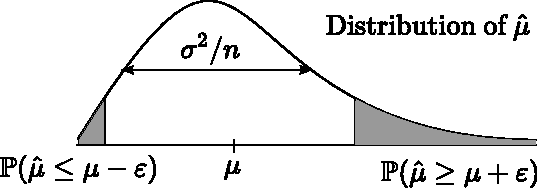
\includegraphics[scale=0.7]{figures/lec02_dist_hat_mu.pdf}
\caption{Distribution of $\hat \mu$ with mean $\mu$ and variance $\sigma^2/n$. The shaded regions denote the upper and lower tails of the distribution for some $\epsilon > 0$.}
\end{figure}

One way is to bound the probability by which $\hat \mu$ differs from the true mean $\mu$. For instance, maybe we want the probabilities of both the tail events to be tiny, so that the probability of $\hat \mu$ not deviating too much from $\mu$ is large:
\begin{align*}
  \PP(\mu \in [\hat \mu - \varepsilon, \hat \mu + \varepsilon]) \geq 1 - (\text{tiny number}) \geq (\text{big number}),
\end{align*}
for some small $\epsilon > 0$.

\subsection*{Central limit theorem (CLT)}
One way to go about bounding the deviation between $\hat \mu$ and $\mu$ is via the central limit theorem. Let $X_1, \ldots, X_n$ be a sequence of iid random variables with zero mean, i.e.\ $\mu = \EE{X_i} = 0$. Let $S_n := \sum_{i=1}^n X_i$ denote the sum of these variables. Let 
\begin{align*}
  Z_n = \frac{S_n}{\sigma \sqrt n} = \frac{S_n}{n} \frac{\sqrt n}{\sigma} = \hat \mu \frac{\sqrt n}{\sigma},
\end{align*}
denote the normalized sum of the random variables. Then as $n \to \infty$, the central limit theorem says that $P_{Z_n} \to P_Z$, where $Z \sim \cN(0, 1)$. \textbf{\textcolor{red}{(What assumptions does CLT need on the distribution of $X_i$s?)}} Recall that for the standard normal distribution, $P_Z(dZ) = \frac{1}{\sqrt{2 \pi}} e^{-z^2/2} dz$. Then,
\begin{align*}
  \PP(\hat \mu \geq \mu + \varepsilon) = \PP( \hat \mu \sqrt n / \sigma \geq \mu + \varepsilon \sqrt n / \sigma ) \stackrel{n \to \infty}{\approx} \PP(Z \geq \mu + \varepsilon \sqrt n / \sigma).
\end{align*}
For the standard normal distribution, not that for any $u > 0$,
\begin{align*}
  \PP(Z \geq u) &= \frac{1}{\sqrt{2 \pi}} \int_{u}^\infty e^{-z^2/2} dz = \frac{1}{\sqrt{2 \pi u^2}} \int_{u}^\infty u \cdot e^{-z^2/2} dz \\
  &\leq \frac{1}{\sqrt{2 \pi u^2}} \int_{u}^\infty z \cdot e^{-z^2/2} dz \tag{since the integral is over the set $\{z > u\}$}\\
  &= \frac{1}{\sqrt{2 \pi u^2}} \big[ - e^{-z^2/2} \big]_u^\infty = \frac{1}{\sqrt{2 \pi u^2}} e^{-u^2/2}.
\end{align*}
Combining the above two results, with $u = \varepsilon \sqrt n / \sigma$, gives 
\begin{align*}
  \PP( \hat \mu \geq \mu + \varepsilon) \lesssim \frac{\sigma}{\sqrt{2 \pi \varepsilon^2 n}} \exp \bigg( \frac{-\varepsilon^2 n}{2 \sigma^2} \bigg).
\end{align*}
Note that this whole argument is not very rigorous, because in order to apply CLT, we need $n \to \infty$, and the above result has a finite $n$. However, the difference between the cumulative density function of $Z_n$ and $Z$ is not too much. (From Berry-Ess\'{e}en theorem, this difference is $\mathcal{O}(\E |X_1|^3/\sqrt n)$.)

\subsection*{Subgaussianity}
We present some useful inequalities for bounding the deviation of a random variables and then discuss how a property called subgaussianity can give very fast decays on tail events. The first is Markov's inequality. For any random variable $X$ and $\epsilon > 0$,
\begin{align*}
  \PP(|X| \geq \varepsilon) \leq \E |X| / \varepsilon. 
\end{align*}
(If the first moment doesn't exist, then this inequality becomes vacuous.) If the second moment exists, then one can derive, using Markov's inequality, the following (known as Chebyshev's inequality):
\begin{align*}
  \PP(|X - \mu| \geq \varepsilon) \leq \VV{X} / \varepsilon^2.
\end{align*}
In general, if the $p$th moment exists, one can obtain $\PP(|X - \mu|^p > \varepsilon) \geq \EE{|X - \mu|^p} / \varepsilon^p$. (It is further possible to optimize for the value of $p \in \NN$ to get the strongest possible inequality, subject to the existence of the $p$th moment.) But we can do something much simpler. Using Markov's inequality we can obtain the following. For a random variable $X$ with $\mu = \EE{X}$ and $\varepsilon > 0$, 
\begin{align*}
  \PP(X \geq \mu + \varepsilon) = \PP(\lambda (X - \mu) \geq \lambda \varepsilon) = \PP( e^{\lambda (X - \mu)} \geq e^{\lambda \varepsilon}) \leq \EE{e^{\lambda (X - \mu)}} / e^{\lambda \varepsilon}, \qquad \text{for all } \lambda > 0.
\end{align*}
Thus, if we can bound the term $\EE{e^{\lambda (X - \mu)}}$, then we can get an exponential decay (which is much faster than what we could obtain by optimizing $p$ in the previous inequalities) on the upper tail event.

\begin{definition}[Subgaussianity]
  A random variable $X$ is called $\sigma$-subgaussian, if $\EE{e^{\lambda (X - \mu)}} \leq e^{\lambda^2 \sigma^2 / 2}$.
\end{definition}
Then by the subgaussianity assumption, we get
\begin{align*}
  \PP(X \geq \mu + \varepsilon) \leq e^{\lambda^2 \sigma^2 / 2 - \lambda \varepsilon} = e^{-\varepsilon^2 / (2 \sigma^2)}.
\end{align*}

(Random remark: If the loss $\ell$ is bounded, then the random variables $L(f_n)$ is also bounded, which means that $L(f_n)$ would be a subgaussian random variable; refer the next lecture.)


\bibliography{all}
% **** THIS ENDS THE EXAMPLES. DON'T DELETE THE FOLLOWING LINE:


\end{document}





